\chapter*{Hardware}
\addcontentsline{toc}{chapter}{Hardware}

\section*{Matrix controller in general}
\addcontentsline{toc}{section}{Matrix controller in general}

Matrix controller implements cellular automaton, it consists of sequential and combinatory parts. Matrix controller connected to processor I/O bus, so its inner parts can communicate with processor through this bus. Also matrix controller connected to clock in order to synchronise acts of reading and modifying its state with processor.

Sequential part consists of matrix buffer, which holds game field state, and status registers  which hold game rules, speed of game and game state (is game running or not). Both matrix buffer and status registers can be read and modified using load/store operations of processor with addresses, specified for this purposes, moreover, whole their status is visible for combinatory part. Matrix buffer, also, can be rewrited all at once by combinatory part.

Combinatory part presented by game processor, it can map current matrix buffer state to next state, depend on status registers content, and provide this new state to matrix buffer.

Also, there is a SR trigger in matrix controller, which processor can set (by accessing specified address) in order to trigger one iteration of the game, it will be reset automaticaly as soon as this iteration end.

We can trigger clearing of whole game field by accessing specified address (no matter for store or for load), this is done by separate AND gate, which true if we access this address and clock is high (this verify, what processor provides valid data).

\begin{figure}[ht]
	\centering
	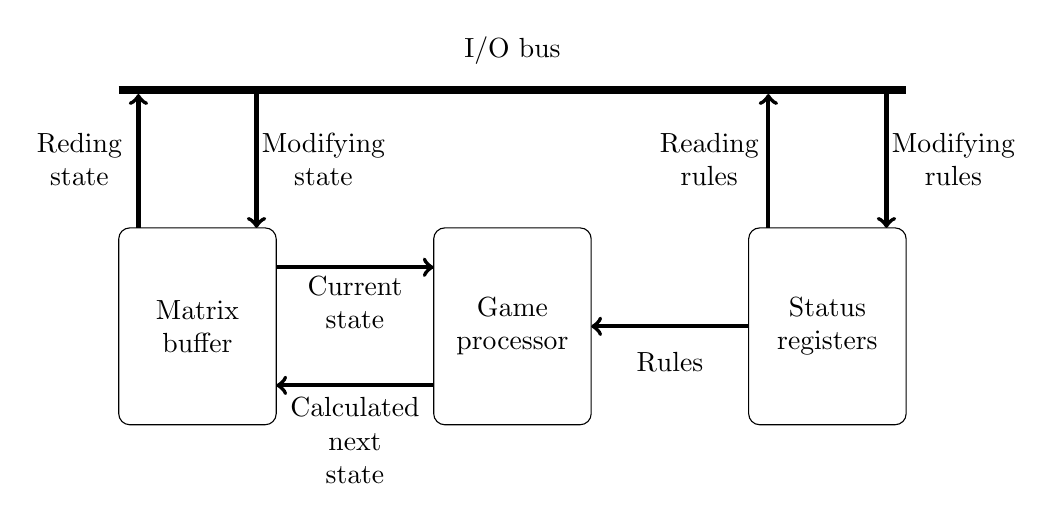
\begin{tikzpicture}[main/.style={draw, rounded corners, minimum width = 20mm, minimum height = 25mm}]
		\node[main, align=center] (buffer) {Matrix\\buffer};
		\node[main, align=center] at (4,0) (processor) {Game\\processor};
		\node[main, align=center] at(8,0) (status) {Status\\registers};

		\node at (4, 3.5) {I/O bus};
		\draw[line width = 3pt] (-1, 3) -- (9, 3);

		\node[align=center] at (-1.5, 2.125) {Reding\\state};
		\path[->, line width = 1.5pt] (-0.75, 1.25) edge (-0.75, 2.95);
		\node[align=center] at (1.6, 2.125) {Modifying\\state};
		\path[->, line width = 1.5pt] (0.75, 2.95) edge (0.75, 1.25);

		\node[align=center] at (6.5, 2.125) {Reading\\rules};
		\path[->, line width = 1.5pt] (7.25, 1.25) edge (7.25, 2.95);
		\node[align=center] at (9.6, 2.125) {Modifying\\rules};
		\path[->, line width = 1.5pt] (8.75, 2.95) edge (8.75, 1.25);

		\node[align = center] at (2, 0.3) {Current\\state};
		\path[->, line width = 1.5pt] (1, 0.75) edge (3, 0.75);
		\node[align = center] at (2, -1.45) {Calculated\\next\\state};
		\path[->, line width = 1.5pt] (3, -0.75) edge (1, -0.75);

		\node at (6, -0.45) {Rules};
		\path[->, line width = 1.5pt] (7, 0) edge (5, 0);
	\end{tikzpicture}
	\caption{Matrix controller}
\end{figure}

\section*{Matrix buffer row}
\addcontentsline{toc}{section}{Matrix buffer row}

Matrix buffer row built around 32-bit register, which holds state of single row of game field (state of 32 cells from this row).

This register is enabled, when game is running and when processor rewrite data in this row. Reasons of it is obvious, we don't need to change anything when the game paused and if processor isn't writing to this row.

Latching new data in this register can be triggered by rising edge of \textbf{clock} (so it will be synchronized with processor) or by rising edge of \textbf{cc} (counter clock from game processor) either (so it will be synchronized with game processor).

Also, because two sources of new state of this row (processor and game processor) changes different amount of bits in state at once (processor changes only first or second 16 bits of state due to size of data bus, game processor can change all 32 bits at once) there is two inputs in this circuit:

\begin{itemize}
	\item \textbf{Narrow in} - 16-bit input from data bus of processor. This source is closed (by controlled buffer) when it's not needed (when there is no writing to this row from processor).
	\item \textbf{Wide in} - input from game processor (new state of this row, calculated by game processor). This source goes straight to the multiplexer.
\end{itemize}

Narrow in (with \textbf{self} - current state of row) goes through block of splitters, which output \textbf{self} with most or least signigicant (depends on 1-bit \textbf{block} input) changed according to narrow input.

If this row is selected for writing from processor - \textbf{narrow in}, combined with \textbf{self} will be source of new state. Otherwise, \textbf{wide in} will be chosen.

Respectively, we have two outputs:

\begin{itemize}
	\item \textbf{Narrow out} - output to data bus of processor. Row will pass its first or second half on this bus (depends on \textbf{block} again) if processor reads data from this row, otherwise it won't pass anything.
	\item \textbf{Wide out} - output to game processor. Row always pass its current state to let game processor calculate its new state if game is running.
\end{itemize}

\section*{Matrix buffer}
\addcontentsline{toc}{section}{Matrix buffer}

Matrix buffer is just 32 \textbf{buffer rows}, connected with each other (for passing signals like \textbf{cc}, \textbf{clock}, \textbf{rd/wr} through all rows). All \textbf{narrow ins} connected to one narrow in input in the south of circuit, which connected to data bus. Also, all \textbf{narrow outs} connected to one narrow out output, connected to data bus.

When processor read or write to some row, decoder select appropriate row and part of this row, using 6-bit address (5 bits specify row and 1 bit specify part - most or least significant 16 bits). Also, \textbf{clock} signal goes only to row, in which processor writes, because only this row needs this signal.

All \textbf{wide ins} are connected to 32 32-bit inputs of matrix buffer, and all \textbf{wide outs} are connected to 32 32-bit outputs of this circuit in order to take/provide whole game field state to game processor.

\section*{Cell}
\addcontentsline{toc}{section}{Cell}

Cell is a single calculator, which calculates new state of single cell, based on its neighbours (actually on amount of alive neighbours), current status of cell and rules.

This is done by two multiplexers, selecting bits from both rules, depend on alive neighbours amount. Selected bits indicate if cell should survive (\textbf{surv} equals 1) or should it become alive (\textbf{born} equals 1). Next state of this cell is calculated according following truth table:

\begin{center}
	\begin{tabular}{|c|c|c|c|}
		\hline
		Surv & Born & State & New \\
		\hline
		0 & 0 & 0 & 0  \\
		\hline
		0 & 0 & 1 & 0 \\
		\hline
		0 & 1 & 0 & 1 \\
		\hline
		0 & 1 & 1 & 1 \\
		\hline
		1 & 0 & 0 & 0 \\
		\hline
		1 & 0 & 1 & 1 \\
		\hline
		1 & 1 & 0 & 1 \\
		\hline
		1 & 1 & 1 & 1 \\
		\hline
	\end{tabular}
\end{center}

This is done with circuit, representing PCNF of this truth table.

\section*{Game processor row}
\addcontentsline{toc}{section}{Game processor row}

This circuit is just 32 cells connected with each other in one row. This circuit have 3 inputs for rows:

\begin{enumerate}
	\item Row \textbf{above} this
	\item Row \textbf{below} this
	\item \textbf{This} row
\end{enumerate}

All of this inputs is \textbf{current} state of this rows.
Also, there is 2 inputs for rules, mentioned before: \textbf{surv} and \textbf{born}.

All of cells 8 \textbf{neighbour} inputs connected to appropriate wires with their neighbours statuses (except leftmost and rightmost cells, which don't have neighbours on the left and on the right respectively).

All of calculated \textbf{new} states of cells goes in single 32 bit wide wire, which goes to the only one output of game processor row - \textbf{new state of this row}.

\section*{Game processor}
\addcontentsline{toc}{section}{Game processor}

Game processors purpose is to calculate new state of whole game field. New state is calculated, based on current, row by row. This is implemented by 5 bit counter, which indicates, which row will be calculated on this tick, and 3 multiplexers choosing appropriate \textbf{this} row, \textbf{above} row and \textbf{below} row for \textbf{game processor row} and 32 "buffering" registers, holding new state until it will be latched in matrix buffer.

Transition of counter value from 31 to 0 meaning, what all 32 row were calculated, causes rising of "equal" out of comparator (which compares counter value and 0), this triggers impulse on \textbf{cc} output and results in matrix buffer latching new state of whole game field.

When game pauses, counter resets to zero, because we need to recalculate whole new game field state after (maybe) something will be changed when game is paused. 

Also, reset of counter is triggered when any of status registers (containing rules of the game) is rewrited, because whole next state should be calculated based on rewrited rules.

\section*{Status registers}
\addcontentsline{toc}{section}{Status registers}

There are two status registers, both of them is conneted to I/O data bus, I/O address bus, rd/wr signal and I/O sel signal (which indicates if processor access I/O address space or not). Reading and writing to this registers can be done with store/load operations of processor with specified addresses. Every writing to this registers will cause reset of game processor counter (see Game processor).

All rules (described here) go from this registers straight to game processor or speed controller.

\section*{One iteration trigger}
\addcontentsline{toc}{section}{One iteration trigger}

For triggering single game iteration SR trigger is used. When its value is 1, it raises \textbf{play} signal for game processor. Setting this trigger to 1 can be triggered by accessing specified address. It will be set to 0 automatically, when game processor calculate new state and matrix buffer latch this new state.

\section*{UART controller}
\addcontentsline{toc}{section}{UART controller}

UART controller contains UART and I/O implementation.

\begin{itemize}
	\item When the processor accesses an address allocated in memory, it writes a character to the UARTa buffer via the data bus or retrieves it from there via the data bus depending on the rd/wr signal.
	\item UART raises the \textbf{dt} signal if a line arrives in the buffer, and the \textbf{con} signal if a remote terminal is connected to the UART. This is used for interrupts triggering, which will be described later.
\end{itemize}

\section*{Interrupt arbiter}
\addcontentsline{toc}{section}{Interrupt arbiter}

The arbiter is circuit, which manages single source of interrupt requests. By connecting arbiters one after another we can assign priority to each interrupt source. This is done with four states arbiter can be in. Each state represent stage of interrupt request trasferring. Here is description of this states:

\begin{enumerate}
	\item \textbf{Zero} - the device does not require interrupts, or it does, but at the moment another device has not finished transmitting its interrupt request. In this state:

		If the device does not require an interrupt, then the IRQ and IAck pass through the arbiter from east to west and from west to east (it should be noted that if the processor is in the \textbf{WAITING} status, its raising of IAck is not considered as a response to the interrupt request, since being in this state, having received an interrupt request, the processor will only return to the \textbf{RUNNING} status, but will not process the request, the request will be processed after the transition to the \textbf{RUNNING} status)

		If the device requires an interrupt, but the other device has not finished transmitting its request, then the IAck output in the east cannot be raised again, but can be lowered (its high level indicates that the other device is transmitting its request)

		The transition from this state to the first is carried out provided that the device requires an interrupt and no other device is transmitting an interrupt request.
	\item The \textbf{first} state is state of sending an interrupt request from the device.
		In this state:

		The IRQ from east to the west and IAck from west to the east are blocked, while the arbiter holds the IRQ output to the west at a high level, signaling the processor that an interrupt is required

		The transition from this state to the second is carried out provided that the processor has responded to the request by raising IAck (which means that the processor state allows the interrupt to be processed)
	\item The \textbf{second} state is state of transfering of the interrupt vector to the processor
		In this state:

		The arbiter still holds the IRQ at a high level, since its lowering will lead to the falling of IAck from processor and termination of the interrupt request transfer process (unlike CdM-8, in which falling of IAck will trigger the interrupt vector latching and completion of interrupt request transfer). In this case, the interrupt vector from the device is fed to the interrupt vector bus connected to the processor. Also, the raised IAck is transmitted to the device to notify it that the processor has responded to its request.

		The transition from this state back to zero and the completion of interrupt processing occurs on the falling edge of the clock, since it is at this moment that the processor latches the interrupt vector and the process of transmitting the request can be considered complete.
\end{enumerate}

\section*{Interrupt bus}
\addcontentsline{toc}{section}{Interrupt bus}

There are two interrupt arbiters, connected to interrupt bus:

\begin{itemize}
	\item The first arbiter manages connection interrupt. It has a higher priority and causes an interrupt when a remote terminal connects, which reflects in rising of a \textbf{con} output of UART.
	\item The second arbiter manages new data interrupt. It has a lower priority and causes an interrupt when a line arrives in the UART buffer, which reflects in rising of \textbf{dt} output of UART. In order to be able to process several lines that arrive one after another or one while the second is being processed, \textbf{dt} output goes through AND gate with negated value of special SR trigger. This trigger take value of 1, when processor answers to new data interrupt request and take value of 0, when processor access specified address (it does this, when single line of input is loaded from UART buffer).
\end{itemize}

